\chapter{Implementazione del sistema}

\section{Schema architetturale completo}
Come si è potuto evincere dal capitolo precedente, il sistema è composto da diverse parti. Ciascuna di esse interagisce con le altre in un modo ben definito. Chiariamo meglio l'architettura completa con uno schema, spiegato nel dettaglio di seguito.
\begin{figure}[h]
\centering
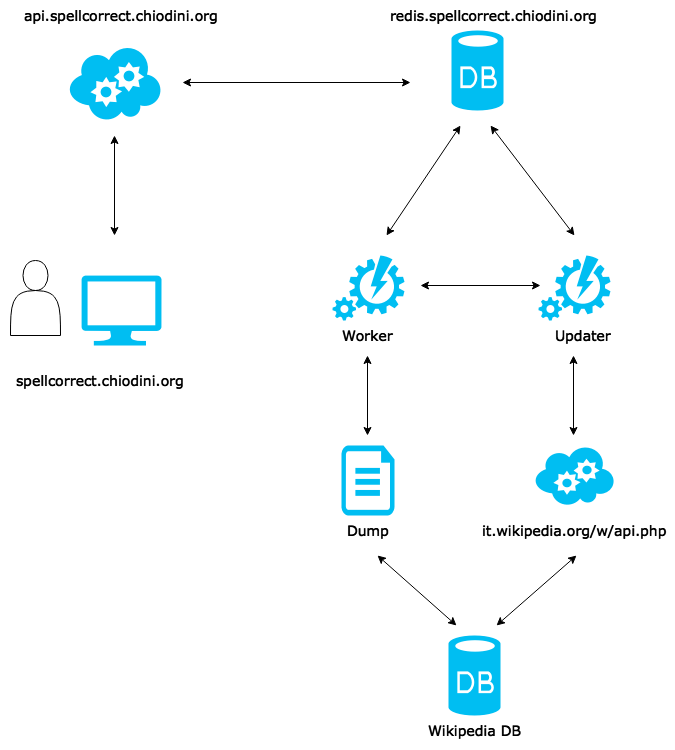
\includegraphics[width=\textwidth]{Figures/architecture.png}
\caption{Architettura del sistema}
\end{figure}

\begin{itemize}
	\item 
\url{spellcorrect.chiodini.org} è servito da Google App Engine\footnote{\url{https://cloud.google.com/appengine/}} ed è costituito da una pagina statica (e alcuni asset). Essa contiene un'area dove l'utente inserisce la parola o la frase da correggere; questa verrà inviata al servizio di API tramite richiesta AJAX.
	\item 
\url{api.spellcorrect.chiodini.org} è una web API, servita sempre da Google App Engine. Essa è tecnicamente realizzata tramite Flask\footnote{\url{http://flask.pocoo.org/}}, un microframework che consente di realizzare un web server usando come linguaggio Python.

La definizione dell'API è semplice: è necessario fare una richiesta a

\makebox[\linewidth]{\texttt{http://api.spellcorrect.chiodini.org/correct/<str>}}
sostituendo \texttt{<str>} con la parola o la frase da correggere. Il servizio risponde nella notazione JSON. Ecco un esempio tipico di risposta:
\begin{lstlisting}[language=json, numbers=none]
{
 "cache": false,
 "corrected": "eccezione", 
 "elapsed_time": "0:00:01.719220",
 "queries": 36,
 "input": "eccezzione"
}
\end{lstlisting}
I campi della risposta hanno i seguenti significati:
\begin{itemize}
\item \texttt{input} contiene l'input ricevuto;
\item \texttt{corrected} contiene la miglior correzione che il sistema è riuscito a calcolare per quell'input;
\item \texttt{elapsed\_time} indica il tempo, con precisione in microsecondi, impiegato per l'elaborazione;
\item \texttt{queries} indica il numero di query effettuate al database Redis;
\item \texttt{cache} indica se la risposta è stata calcolata al momento oppure recuperata dalla cache (cfr. \ref{cache}).
\end{itemize}

\item
\url{redis.spellcorrect.chiodini.org} ospita il DBMS Redis che si mette in ascolto sulla porta \texttt{TCP/6379}. Il DBMS è stato installato su una VPS (cfr. \ref{dbms}). 

\item
La restante parte dello schema rappresenta quanto già ampiamente discusso nel capitolo precedente. Le frequenze iniziali vengono memorizzate in Redis dopo essere state ottenute elaborando il dump. Gli aggiornamenti continui sono invece realizzati tramite un modulo (``Updater'' nello schema in figura) che periodicamente interroga le API di Wikipedia e processa le eventuali modifiche delle frequenze inviandole sempre a Redis.
\end{itemize}

\section{Algoritmo}
L'algoritmo di base è tratto da un articolo di Peter Norvig \cite{norvig}, che è l'attuale direttore del dipartimento di Ricerca presso Google. Rispetto alla versione originale sono stati modificati diversi punti, in accordo alla teoria definita nel capitolo \ref{cap_teoria}.

Lo schema riporta i passi essenziali dell'algoritmo di correzione:
\begin{itemize}
\item L'input viene ricevuto dall'applicazione Flask.
\item Per ciascuna parola presente nell'input, si procede alla generazione di tutte le parole candidate a sostituire quella presente. Per fare ciò, all'avvio viene precaricato in memoria tutto il dizionario delle parole conosciute. Tutte le parole presenti nel dizionario, aventi una distanza di  Damerau–Levenshtein (cfr. \ref{distanzadameraulev}) inferiore o uguale a due rispetto all'input, vengono considerate possibili candidati.
\item Per ogni candidato vengono effettuate tre query al database che misurano la probabilità del candidato di per sè e quella rispetto alla parola precedente e seguente (naturalmente ove applicabile). Viene inoltre considerata anche la probabilità basata sulla distanza Damerau–Levenshtein a cui la parola si trova rispetto a quella originale. Per un approccio rigoroso, si riveda il paragrafo \ref{probabilita}.
\item Il candidato con la probabilità più alta viene considerato il migliore e restituito come soluzione. È importante notare che anche la parola stessa originaria costituisce un candidato: essa infatti potrebbe essere corretta e non necessitare di alcuna alterazione.
\end{itemize}
\begin{figure}[h]
\centering
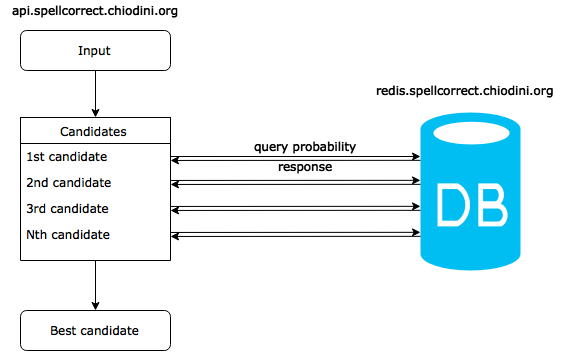
\includegraphics[width=\textwidth]{Figures/original_algorithm.png}
\caption{Algoritmo in dettaglio}
\label{fig:algoritmo}
\end{figure}

\pagebreak

\section{Efficienza}
I paragrafi seguenti spiegano i principali accorgimenti che sono stati adottati per rendere il sistema il più efficiente possibile.

\subsection{Ottimizzazione dell'algoritmo}
A un lettore attento non sarà sfuggito che l'algoritmo mostrato in figura \ref{fig:algoritmo} esegue un gran numero di interrogazioni sul database. Poiché client e server sono due host distinti, ogni query avrà un tempo di esecuzione pari alla latenza tra i due host sommata al tempo di esecuzione dell'interrogazione stessa. 

Redis è in grado di rispondere a una query in un tempo quasi sempre inferiore al millisecondo, ma la latenza tra due host su una rete geografica può essere anche 100 volte tanto. Essendo molto alto il numero delle interrogazioni è necessario evitare che per ciascuna sia necessario lo scambio di pacchetti TCP andata e ritorno: ciò porta a tempi di risposta complessivi inaccettabili.

Per risolvere il problema e ridurre drasticamente il tempo complessivo di risposta sfruttiamo una funzionalità di Redis, ``pipeline'', che consente di bufferizzare le query ed eseguirle tutte in un'unica volta.

Supponiamo che per correggere una certa frase servano 5000 query, che la latenza tra i due host sia di 50 ms e che Redis risponda a tutte le query in 1 ms: la tabella mostra un confronto tra i tempi dei due algoritmi.
\begin{table}[h]
\centering
\begin{tabular}{lrrl}
\toprule
Metodo		&	Latenza TCP					&	Tempo query		&	Tempo globale	\\
\midrule
Originale	&	$5000 \cdot 2 \cdot 50$ ms& $5000 \cdot 1$ ms	&	$\sim$ 8 min		\\
Ottimizzato	&	$1 \cdot 2 \cdot 50$ ms		& $5000 \cdot 1$ ms	&	$\sim$ 5 sec		\\
\bottomrule
\end{tabular}
\caption{Confronto tra i tempi di risposta dei due algoritmi}
\end{table}

\begin{figure}[h]
\centering
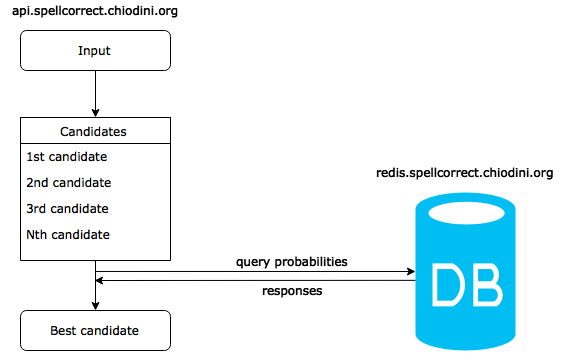
\includegraphics[width=\textwidth]{Figures/improved_algorithm.png}
\caption{Algoritmo ottimizzato}
\end{figure}
\subsection{Cache}
\label{cache}
Poiché più persone potrebbero richiedere la correzione delle stesse parole nel giro di poco tempo, ha senso mantenere una cache dei risultati. Questo permette di evitare il ricalcolo delle probabilità, che risulta essere molto oneroso.

All'interno della piattaforma App Engine è possibile sfruttare Memcached\footnote{\url{http://memcached.org/}}, un sistema distribuito ad alte prestazioni per salvare in memoria oggetti. Per quanto il progetto Memcached nasca e resti generico, esso è frequentemente impiegato come meccanismo di cache per alleviare il carico del database e velocizzare applicazioni web dinamiche e servizi di API.

Il funzionamento è tanto potente quanto semplice. Memcached prevede una chiave (in questo caso l'input), un valore (salviamo l'intero oggetto della risposta) e una scadenza. Ad ogni chiamata all'API viene eseguito questo codice (riportato nella sua versione essenziale):
\begin{lstlisting}[language=Python, numbers=none]
# Try to save resources and reduce response time retrieving
# the answer from the cache.
res = memcache.get(words_str)

# If the response has not been found in the cache:
if res is None:

    # Compute it.
    res = self.parse(words_str)
    
    # Add it to the cache (expire time 1 day).
    memcache.add(words_str, res, 86400)
\end{lstlisting}
\subsection{Scalabilità}
Oltre alle misure descritte nei due paragrafi precedenti si è ritenuto opportuno tenere in considerazione particolare la scalabilità del servizio di API. La piattaforma di produzione scelta, Google App Engine, consente infatti di lavorare sul concetto di istanza per garantire alta affidabilità ed elevate prestazioni.

Il meccanismo è semplice: la piattaforma monitora continuamente svariati parametri sulle risposte fornite dall'applicazione, di cui il più importante è il tempo medio di risposta. Quando quest'ultimo valore aumenta oltre una soglia ritenuta inaccettabile è evidente che un'instanza dell'applicazione non è sufficiente a soddisfare il carico corrente sul server e ne viene pertanto lanciata un'altra. In modo analogo, quando l'utilizzo medio delle risorse di un'instanza (CPU, RAM) diventa irrisorio App Engine decide di terminare l'istanza riducendo il costo complessivo.

Tutti i parametri di configurazione relativi alle istanze sono manipolabili nel file \texttt{app.yaml} e includono, oltre a quanto già visto, la scelta delle caratteristiche hardware virtuali dell'istanza e la possibilità di averne un certo numero sempre attive, pronte a rispondere alle richieste.